% Important: The shell-escape flag is required for the Minted package.
% Please compile this document with 'pdflatex -shell-escape main.tex'.
% If you are using another IDE, you may be able to specify this in the
% options or to provide an option like '% !TEX option = -shell-escape'
% in this file, depending on your builder. See the README.md for more.

% Don't put any content in here.
% Don't even include content files by using \input or \inlcude.
% Put your content into components/text.tex or include it there using \input.
% You probably want to modify the following files:
%   components/info.tex             contains the author, title etc.
%   components/settings.tex         contains the packages and settings.
%   components/commands.tex         contains helpful custom commands.
%   components/glossary.tex         contains an explanation of the used terms.
%   components/acknowledgements.tex contains the acknowledgements.
%   components/quote.tex            contains a quote.
%   components/abstract.tex         contains the abstract of the document.
%   components/text.tex             includes the actual content of the document.
%   components/outline.tex          contains the outline.
%   components/preface.tex          contains the preface.
%   chapters/                       contains the main text.
%   bibliography/literature.bib     contains the BibTeX entries.
%   images/                         contains all your content-related images.
%
% You probably don't need to change anything in the following files:
%   components/cover.tex            formats the front cover of the document.
%   components/titlepage.tex        formats the title page of the document.
%   components/disclaimer.tex       formats the disclaimer page.
%   styles/                         contains style elements (e.g. logos).
%   main.tex                        contains the top-level code structure.
%   README.md                       contains information about this template.

\documentclass[11pt,
              a4paper,
              article,
              index=totoc,
              headsepline,
              footsepline,
              BCOR=12mm,
              dvipsnames,
              DIV=13]{scrbook}
\setcounter{secnumdepth}{3}
\usepackage{amsthm}
\usepackage[ruled,vlined]{algorithm2e}
\usepackage{tikz}
\usepackage{wrapfig}
\usetikzlibrary{shapes,arrows,positioning}
\setlength{\parindent}{0pt}
\setlength{\parskip}{6pt}
\usepackage{caption}
\usepackage{subcaption}
\usepackage{adjustbox}
\usepackage{acronym}
\usepackage{hyperref}[2011/02/05]

\makeatletter
\AtBeginDocument{%
  \renewcommand*{\AC@hyperlink}[2]{#2}%
}
\makeatother

% KOMA scrbook options:
%  index=totoc: include an entry for the index in the table of contents.
%  headsepline: use horizontal line under heading.
%  footsepline: use horizontal line above footer.
%  BCOR: binding correction (e.g.: BCOR=12mm)
%  DIV: Number of sheet sections (used for layout) (e.g.: DIV=13)


%  This code base is currently hosted at: 
%  https://github.com/waltsims/TUM_Thesis_Template_CSE
\usepackage[backend=biber, sorting=none]{biblatex}
\addbibresource{bibliography/literature.bib}
% !TEX root = ../main.tex
% Set here the title, authors and other stuff to be used for the cover
% This file is used by MAIN.TEX

% set title, authors and stuff for the cover
\def\university{Technical University of Munich}
\def\department{School of Computation, Information and Technology - Informatics}
\def\universityLogo{styles/tum_logo}
\def\program{Robotics, Cognition, Intelligence (M.Sc.)}
\def\programLogo{styles/cse_logo}
\def\doctype{Master's Thesis in Robotics, Cognition, Intelligence}

\def\title{Active Critic in Partially Observable Markov Decision Processes}
\def\titleger{Aktiver Kritiker in teilweise beobachtbaren Markov-Entscheidungsprozessen}
\def\author{Hendrik Elvers}
\def\supervisor{Prof. Dr.-Ing. habil. Alois Knoll}
\def\advisor{Dr. rer. nat. Zhenshan Bing}
\def\date{April 15th, 2023}

\def\keywords{{RL}, {IL}, {POMDP}, {MDP}}

% The following are used for the PDF metadata, by default the same as above.
\def\metaTitle{\title}
\def\metaAuthor{\author}
\def\metaSubject{\doctype\ -\ \university}
\def\metaKeywords{\keywords}

% text to appear in the footer
\def\footertext{}


\input{components/settings}

\input{components/commands}

\input{components/glossary}

\makeglossaries

\begin{document} 

\begin{figure}[htbp]
  \centering
  \begin{subfigure}[t]{0.32\textwidth}
    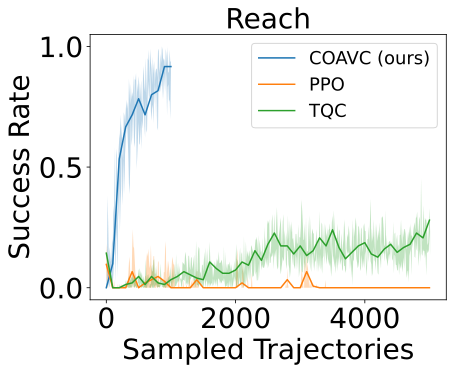
\includegraphics[width=\textwidth]{images/dense_1_big_font/Reach.pdf}
    \caption{One expert demonstration.}
  \end{subfigure}
  \begin{subfigure}[t]{0.32\textwidth}
    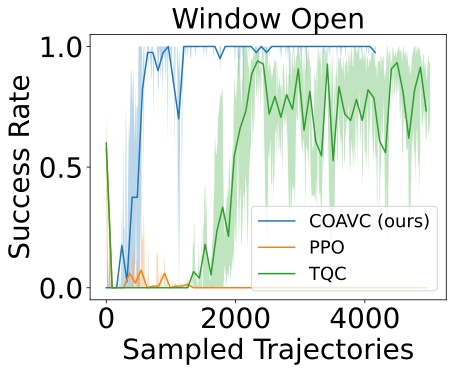
\includegraphics[width=\textwidth]{images/dense_1/Window Open.pdf}
    \caption{One expert demonstration.}
  \end{subfigure}
  \begin{subfigure}[t]{0.32\textwidth}
    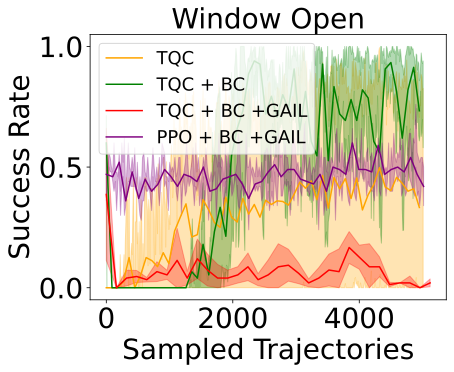
\includegraphics[width=\textwidth]{images/TQC_bc_GAIL_vs_ref/Window Open.pdf}
    \caption{Comparison between tqc with no expert demonstrations and expert guided baselines.}
    \label{fig:TQC_0_vs_exp}
  \end{subfigure}

  \begin{subfigure}[t]{0.32\textwidth}
    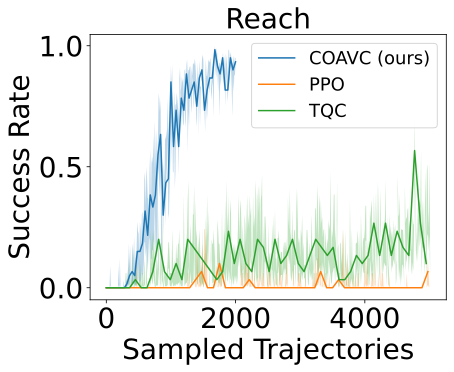
\includegraphics[width=\textwidth]{images/dense_0/Reach.pdf}
    \caption{No expert demonstrations.}
  \end{subfigure}
  \begin{subfigure}[t]{0.32\textwidth}
    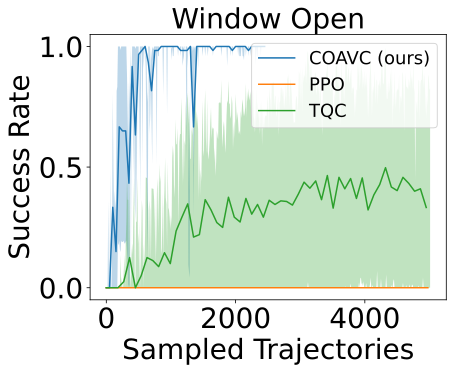
\includegraphics[width=\textwidth]{images/dense_0/Window Open.pdf}
    \caption{No expert demonstrations.}
  \end{subfigure}
  \begin{subfigure}[t]{0.32\textwidth}
    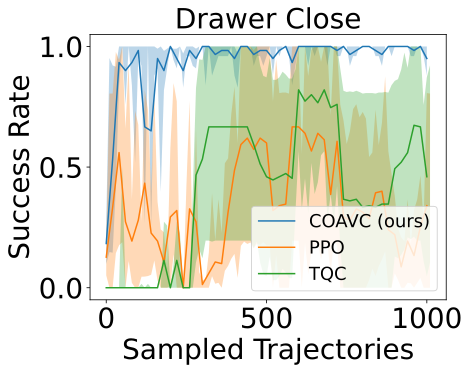
\includegraphics[width=\textwidth]{images/dense_0/Drawer Close.pdf}
    \caption{No expert demonstrations.}
  \end{subfigure}

  \caption{\textbf{Continued Observation}. All baselines were pretrained using behavioral cloning with the given number of expert demonstrations. 
    The x-axis shows the number of sampled environment episodes, each with 100 steps. 
    Continued observations and a sparse reward signal at the end of each episode was provided. 
    The shaded area indicates the standard deviations from three runs per experiment.}
    \label{fig:dense_ref}
\end{figure}
  
\end{document}
